\subsection{Základy kryptografie, RSA, DES}

\subsubsection*{Základy kryptografie}
TODO

\subsubsection*{RSA (Rivest-Shamir-Adleman)}
Asymetrická šifra (různé klíče pro šifrování a dešifrování), použitelná jako šifra s veřejným klíčem.

\textbf{Inicializace:}
\begin{penumerate}
	\item vybrat dvě dostatečně velká prvočísla $p$, $q$
	\item $n:= p\cdot q$
	\item spočítat totient: $\varphi(n) := (p-1)\cdot (q-1)$\\ 
	(Eulerův totient $\varphi(n)$ je počet čísel menších než $n$, která jsou s $n$ nesoudělná)
	\item vybrat $e$ takové, že $1 < e < \varphi(n)$ a $e$ je nesoudělné s $\varphi(n)$\\ -- $e$ bude \emph{veřejný klíč (public key)}
	\item vybrat $d$ tak, aby 
		$$d\cdot e \equiv 1 \mod \varphi(n)$$ 
		takové $d$ lze najít rozšířeným euklidovým algoritmem\\
		-- $d$ bude \emph{dešifrovací klíč (private key)}
\end{penumerate}

\textbf{Šifrování:}
\begin{penumerate}
	\item Alice posílá public key Bobovi (čísla $n$ a $e$), nechává si private key
	\item Bob chce Alici poslat zprávu $m$ (musí být převedena na celé číslo $m < n$)
	\item Bob spočítá :
		$$c = m^e \mod n$$
	\item Bob odešle $c$ Alici
\end{penumerate}

\textbf{Dešifrování:}
\begin{penumerate}
\item Alice přijala $c$
\item Spočítá:
	$$m = c^d \mod n$$
\end{penumerate}

Šifra (to, že to vůbec funguje, tedy, že $m = (m^e)^d$) se opírá o několik netriviálních vět algebry...

\subsubsection*{DES (Data Encryption Standard)}
\begin{pitemize}
\item bloková šifra (vstup plaintext - 64bitů, výstup ciphertext 64bitů)
\item symetrický klíč (stejný pro šifrování i dešifrování) -- strany si ho musí vyměnit po bezpečném kanále
\item klíč -- 64bitů, z nich se používá ale pouze 56bitů (zbytek se zahodí nebo funguje jako kontrola parity)
\item původně implementována hardwarem
\item stejný algoritmus (i hardware) použitý jak pro šifrování, tak pro dešifrování
\end{pitemize}

\begin{figure}[ht]
  \begin{center}
    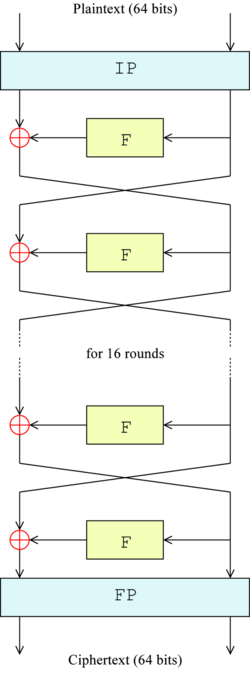
\includegraphics[width=5cm, angle=90]{informatika/siete_a_bezpecnost/obrazky/des-main-network.png}
    \caption{Schéma hlavní sítě algoritmu DES}
  \end{center}
\end{figure}

\begin{obecne}{Šifrování:}
\begin{pitemize}
	\item vstup projde iniciální permutací (IP:64b $\rightarrow$ 64b), na konci probíhá inverzní finální permutace (FP), následuje 16 identických kol šifrování:
	\item blok 64 bitů se rozdělí na dvě půlky po 32bitech, 
	\begin{pitemize}
		\item pravá půlka slouží jako vstup pro funkci F a také je v dalším kole použita jako levá část
		\item levá půlka se xoruje s výstupem funkce F a výsledek je použit v dalším kole jako pravá část
	\end{pitemize}
	\item celý cyklus se provede 16x a v závěru se ještě aplikuje finální permutace
\end{pitemize}
\end{obecne}

\begin{figure}[ht]
  \begin{center}
    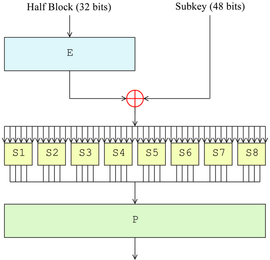
\includegraphics[width=6cm]{informatika/siete_a_bezpecnost/obrazky/des-f-function.png}
    \caption{Funkce \emph{F} v algoritmu DES}
  \end{center}
\end{figure}

\begin{obecne}{Funkce F:}
\begin{pitemize}
	\item ve funkci F probíhá míchání s klíčem. V každém kole vstupuje do funkce F 32bitů z \uv{pravé půlky} a 48bitový subklíč (odvozen z 56bitového klíče, detaily později).
	\item 32bitů z pravé půlky je nejprve expandováno na 48 bitů (fixní expanzní permutací, na obrázku označena E), potom xorováno se subklíčem. 
	\item Výsledek xorování se rozdělí na 8 bloků po 6bitech. Každý blok je pak vstupem jedné z osmi S funkcí. Každá S funkce převádí 6 bitů na 4 bity (nelineární transformací, \uv{zadrátované}).
	\item Výstupy S funkcí se opět spojí do jednoho bloku (8x4 = 32bitů) -- to je výsledek celé funkce F.
\end{pitemize}
\end{obecne}

\begin{obecne}{Dešifrování:} 
Díky prohazování poloviček v jednotlivých kolech lze dešifrování provádět stejnou funkcí (na stejném hardwaru), jako šifrování. Pouze je potřeba používat subklíče v opačném pořadí.
\end{obecne}

\begin{figure}[ht]
  \begin{center}
    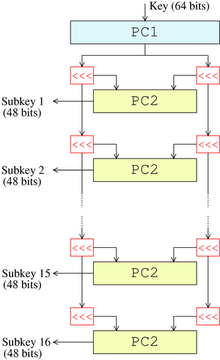
\includegraphics[width=6cm]{informatika/siete_a_bezpecnost/obrazky/des-key-schedule.png}
    \caption{Subklíče v algoritmu DES}
  \end{center}
\end{figure}

\begin{obecne}{Subklíče:}
\begin{pitemize}
	\item protože je klíč původně 64bitový, ale ve skutečnosti se používá pouze 56bitů (ostatní se zahazují, nebo slouží pro kontrolu parity), nejprve je vybráno těchto 56bitů funkcí PC1 (Permuted Choice 1) 
	\item Dále se vždy pro každé kolo 56 bitů rozdělí na dvě půlky po 28bitech. Každá z těchto půlek se bitově posune doleva (o jeden nebo dva bity, to je pevně určeno pro každé kolo). Takto posunuté půlky se vloží jako vstup funkce PC2, která vygeneruje 48bitový subklíč. Obě půlky také slouží jako vstup pro další kolo. 
	\item Algoritmus zaručuje, že každý bit z původního 56bitového klíče je použit asi ve 14-ti ze 16-ti subklíčů. 
	\item Pro dešifrování se klíče musí generovat v opačném pořadí (místo doleva se posouvá doprava).
\end{pitemize}
\end{obecne}
